\documentclass{beamer}
\usepackage{lsfolien}
\usepackage{enumitem}
\usepackage[main=german,russian]{babel}

\title{Modellierung nachhaltiger Systeme\\ und Semantic Web\\[6pt] Technische
  Systeme bei (Koltze, Souchkov)}

\author{Hans-Gert Gr\"abe}

\date{10. November 2020}

\begin{document}
\begin{frame}
  \maketitle
\end{frame}

\begin{frame}{Gesetz, Gesetzmäßigkeit, Trend ... oder was?}
  \begin{itemize}[label={$\bullet$},itemsep=1em]
  \item Was evolviert? Wie lassen sich Kontinuitätslinien im Entstehen und
    Vergehen realer technischer Systeme markieren?
  \item Wie wird dieselbe Frage in der Biologie gelöst?
  \item Wie kann überhaupt Wesentliches von Unwesentlichem geschieden werden?
  \item Was hat es mit \emph{Wesen} und \emph{Erscheinung} auf sich?
  \end{itemize}
\end{frame}

\begin{frame}{Altschullers Entwicklungsgesetze}

Altschuller hat acht solcher Gesetze identifiziert und genauer besprochen.
\small
\begin{enumerate}
\item[A1] \textbf{Gesetz der Vollständigkeit der Teile eines Systems:}
  Notwendige Bedingungen für die Lebensfähigkeit eines technischen Systems ist
  das Vorliegen der Hauptteile des Systems und eine minimale
  Funktionsfähigkeit derselben.
\item[A2] \textbf{Gesetz der „energetischen Leitfähigkeit“ eines Systems:}
  Eine notwendige Bedingung für die Lebensfähigkeit eines technischen Systems
  ist der Energiefluss durch alle Teile des Systems.
\item[A3] \textbf{Gesetz der Abstimmung der Rhythmik der Teile eines Systems:}
  Eine notwendige Bedingungen für die Lebensfähigkeit eines technischen
  Systems ist die Abstimmung der Rhythmik (der Schwingungsfrequenzen, der
  Periodizität) aller Teile des Systems.
\item[A4] \textbf{Gesetz der Erhöhung des Grades der Idealität eines Systems:}
  Die Entwicklung aller Systeme verläuft in Richtung auf die Erhöhung des
  Grades der Idealität.
\end{enumerate}
\end{frame}

\begin{frame}{Altschullers Entwicklungsgesetze}
  \small
\begin{enumerate}
\item[A5] \textbf{Gesetz der Ungleichmäßigkeit der Entwicklung der Teile eines
  Systems:} Die Entwicklung der Teile eines Systems erfolgt ungleichmäßig. Je
  komplizierter das System ist, umso umgleichmäßiger verläuft die Entwicklung
  seiner Teile.
\item[A6] \textbf{Gesetz des Übergangs in ein Obersystem:} Nach Erschöpfung
  seiner Entwicklungsmöglichkeiten wird ein System als Teil in ein Obersystem
  aufgenommen. Dabei erfolgt die weitere Entwicklung auf der Ebene des
  Obersystems.
\item[A7] \textbf{Gesetz des Übergangs von der Makro- zur Mikroebene:} Die
  Entwicklung der Arbeitsorgane eines Systems erfolgt zunächst auf der
  Makroebene und anschließend auf der Mikroebene.
\item[A8] \textbf{Gesetz der Erhöhung des Anteils von Stoff-Feld-Systemen:}
  Die Entwicklung technischer Systeme verläuft in Richtung auf die Erhöhung
  des Anteils und der Rolle von Stoff-Feld-Wechselwirkungen.
\end{enumerate}
\end{frame}

\begin{frame}{Evolution technischer Systeme bei (Koltze, Souchkov)}
  
Dort werden \emph{Gesetze} und \emph{Trends} unterschieden.\vskip1em

\textbf{5 Gesetze:} G1=A1, G3=A4, G4=A5, G5=A8,\\ ein \emph{Gesetz (G2) der
  Vollständigkeit des Obersystems} \vskip1em

\textbf{11 Trends}\vspace{.5em}
\begin{itemize}
\item[T1] Dynamisierung
\item[T2] Koordination und Evolution der Rhythmik (A3, aber ergänzt um einen
  Evolutionsgedanken)
\item[T3] Gestalt- und Formkoordination
\item[T4] Evolution der Geometrie
\item[T5] Erhöhung des Energie-Leitvermögens (A2, aber nicht nur die
  \emph{Existenz} entsprechender Flüsse wird thematisiert, sondern auch die
  \emph{Intensivierung} dieser Flüsse)
\end{itemize}
\end{frame}

\begin{frame}{Evolution technischer Systeme bei (Koltze, Souchkov)}
\begin{itemize}
\item[T6] Übergang auf die Mikroebene (A7)
\item[T7] Zunehmende Steuerbarkeit 
\item[T8] Erhöhung der Automation 
\item[T9] Übergang zum Obersystem (A6)
\item[T10] Zusammenfall 
\end{itemize}
\vskip1em
In einer Abbildung dann noch zusätzlich
\begin{itemize}[noitemsep]
\item[T11] Steigerung des Grads der Kontrolle
\item[T12] Funktionale Evolution
\end{itemize}
Einer zuviel? In der Übersicht fehlt T9=A6.
\vskip1em

Trends sind in jener Abbildung weiter in \textbf{26 Entwicklungslinien}
untergliedert.
\end{frame}

\begin{frame}{Gesetze, Trends, Entwicklungslinien}

Altschuller unterscheidet\vspace{.5em}
\begin{itemize}[label=$\bullet$]
\item statische Gesetze („die die Anfangsperiode im Leben technischer Systeme
  bestimmen“)
\item kinematische Gesetze („die die Entwicklung technischer Systeme
  bestimmen, unabhängig von speziellen technischen und physikalischen
  Faktoren“) und
\item dynamische Gesetze („der Entwicklung moderner technischer Systeme unter
  der Wirkung konkreter technischer und physikalischer Faktoren“)
\end{itemize}
\vskip1em\small \emph{Statische und kinematische Gesetze} sind nach
Altschuller universell, „zeitlos“ („sie gelten zu allen Zeiten, nicht nur für
technische Systeme, sondern für Systeme überhaupt“), \emph{dynamische Gesetze}
haben dagegen einen eher speziellen Charakter („sie widerspiegeln die
Hauptentwick- lungstendenzen der technischen Systeme speziell in unserer
Zeit“).

\end{frame}

\begin{frame}{Gesetze, Trends, Entwicklungslinien}

Begriffliches Fundament von V. Petrov:\vskip1em\small

Ein \textbf{Gesetz} ist ein notwendiges, wesentliches, nachhaltiges, sich
wiederholendes Phänomen.\medskip

Ein Gesetz drückt eine Beziehung zwischen Gegenständen, den Bestandteilen
dieses Gegenstands, zwischen den Eigenschaften von Dingen als auch zwischen
den Eigenschaften innerhalb dieser Dinge aus.\medskip

Aber nicht alle Beziehungen sind Gesetze. Beziehungen können notwendig und
zufällig sein.  Ein Gesetz ist eine \textbf{notwendige Beziehung}.\medskip

Es bringt die wesentliche Beziehung zwischen im Raum koexistierenden Dingen
zum Ausdruck. Es ist ein Gesetz des Funktionierens.  Gesetze existieren
\emph{objektiv}, unabhängig vom Bewusstsein der Menschen.\medskip

Eine \textbf{Gesetzmäßigkeit} ist eine durch objektive Gesetze induzierte
Bedingtheit; eine Form, in der sich die Existenz und Entwicklung in
Übereinstimmung mit den Gesetzen entfaltet,
\end{frame}

\begin{frame}{Ein Modell der Evolution technischer Systeme}

(Koltze, Souchkov) präsentieren ein Modell der Entwicklung technischer Systeme
  längs S-Kurven. 
  \begin{center}
    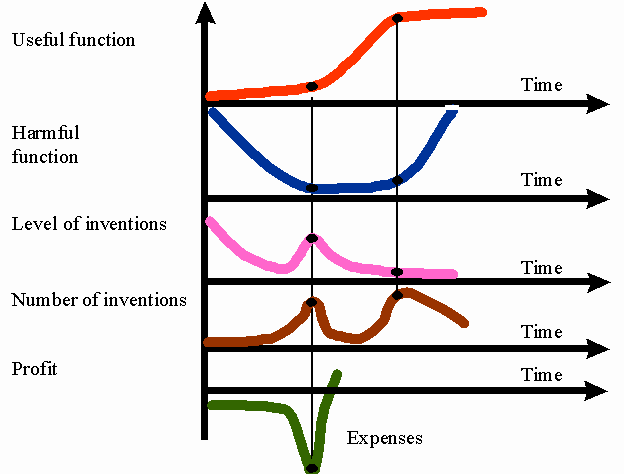
\includegraphics[width=.8\textwidth]{SCurve-3.png}
  \end{center}
\end{frame}

\begin{frame}{Das S-Kurven-Modell}
  \begin{center}
    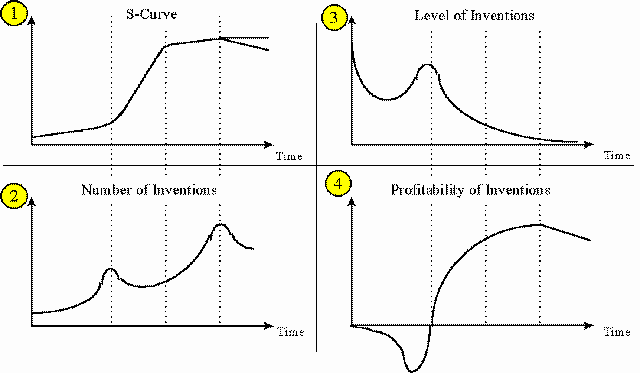
\includegraphics[width=\textwidth]{SCurve-4.png}
  \end{center}
\end{frame}
\begin{frame}{Das S-Kurven-Modell}
\small
Das Modell besteht aus\vskip1em 
\begin{itemize}[label=$\bullet$,noitemsep]
\item einer monoton wachsenden Funktion $f(t)$, „Grad der Systemleistung
  (Hauptparameter der Wertschöpfung) basierend auf einem gegebenen Prinzip“.
\item einer „Glockenkurve“ $g(t)$, „Aufwand (Material, Energie, Personal, FuE)
  zur Wertschöpfung und Lieferung der Funktionalität“),
\item einer „Rentabilitäts-Kurve“ $r(t)$ und 
\item einer Kurve $n(t)$ des „Niveaus der Ideen“. 
\end{itemize}

Diese Kurven bilden die Grundlage, die Evolution in \textbf{drei Phasen} zu
unterteilen, die Phasen
\begin{itemize}[label=$\bullet$,noitemsep]
\item \textbf{Geburt des Systems} -- Erschaffung der Hauptfunktion,
\item \textbf{Wachstum} -- Wachstum der Hauptfunktion,
\item \textbf{Reife und Zusammenfall} -- Bewahrung der Hauptfunktion. 
\end{itemize}
\end{frame}
\begin{frame}{Das S-Kurven-Modell}
  \begin{center}
    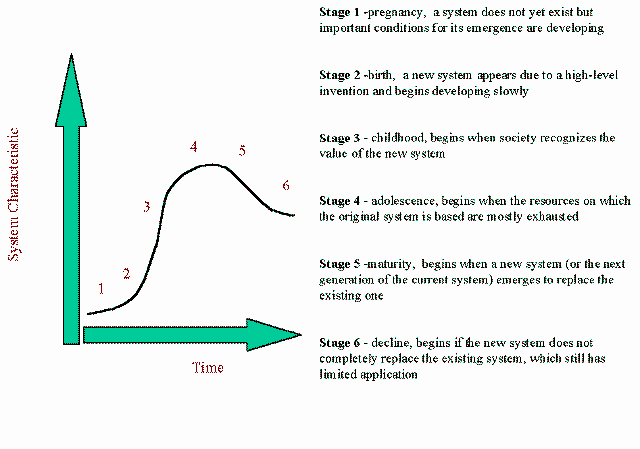
\includegraphics[width=\textwidth]{SCurve-5.png}
  \end{center}
\end{frame}
\end{document}
